\documentclass[a4paper]{article}

\usepackage{fullpage} % Package to use full page
\usepackage{parskip} % Package to tweak paragraph skipping
\usepackage{tikz} % Package for drawing
\usepackage{amsmath}
\usepackage{hyperref}
\usepackage{verbatimbox}
\usepackage{listings}
\usepackage{xcolor}
\usepackage{subfigure}

\definecolor{mygreen}{rgb}{0,0.6,0}
\definecolor{mygray}{rgb}{0.5,0.5,0.5}
\definecolor{mymauve}{rgb}{0.58,0,0.82}
\lstset{ %
  backgroundcolor=\color{white},   % choose the background color
  basicstyle=\footnotesize,        % size of fonts used for the code
  numberstyle=\tiny,
  breaklines=true,                 % automatic line breaking only at whitespace
  captionpos=b,                    % sets the caption-position to bottom
  commentstyle=\color{mygreen},    % comment style
  escapeinside={\%*}{*)},          % if you want to add LaTeX within your code
  keywordstyle=\color{blue},       % keyword style
  stringstyle=\color{mymauve},     % string literal style
}

\title{CSCE 569: Homework 2}
\author{Nick Tyler}
\date{03/02/18}

\begin{document}

\maketitle

\section*{Jacobi Iterative Method}
To parallelize the jacobi method, each iteration of the while loop was parallelized.  Inside the parallel region the loop to copy the matrix is parallelized as well as the main computational loop. For the computational loop a reduction was added to get the correct error. After the computational loop a single section is placed in the loop to print and calculate the error and k properly.

\begin{lstlisting}[language=C++]
while ((k <= mits) && (error > tol)) {
  error = 0.0;
#pragma omp parallel
  {
/* Copy new solution into old */
#pragma omp for private(i, j)
   for (i = 0; i < n; i++)
     for (j = 0; j < m; j++)
       uold[i][j] = u[i][j];
#pragma omp for private(i, j) reduction(+ : error)
   for (i = 1; i < (n - 1); i++) {
     for (j = 1; j < (m - 1); j++) {
       resid = (ax * (uold[i - 1][j] + uold[i + 1][j]) +
               ay * (uold[i][j - 1] + uold[i][j + 1]) + b * uold[i][j] -
               f[i][j]) / b;

       u[i][j] = uold[i][j] - omega * resid;
       error = error + resid * resid;
      }
   }
#pragma omp single nowait
   {
     if (k % 500 == 0)
       printf("Finished %ld iteration with error: %g\n", k, error);

     error = sqrt(error) / (n * m);
     k = k + 1;
    }
  } // End omp parallel region
}
\end{lstlisting}


\section*{Histogram}
To parallelize the histogram I made a temporary two dimensional array so that each thread could have it's own histogram array. This made sure that each thread could write to the histogram array without issues. The temporary array is first zeroed with a for loop for each thread. Then the image is looped over in a parallel loop. Once the image is looped over the actual histogram array is filled in a omp single loop to make sure the histogram is filled properly. Then the normalization is done with a max reduction loop and a parallel loop to divide by the max.

\begin{lstlisting}[language=C++]
int max_threads = omp_get_max_threads();
float temp[MAX_SIZE][max_threads];
#pragma omp parallel private(i, j, k, x, t) shared(temp)
{
  int thread = omp_get_thread_num();
  for (x = 0; x < MAX_SIZE; x++)
    temp[x][thread] = 0;
#pragma omp for reduction(+ : temp)
  for (i = 0; i < src.cols; i++) {
    for (j = 0; j < src.rows; j++) {
      k = src.at<uchar>(j, i);
      temp[k][thread] += 1;
    }
  }
#pragma omp single
  for (t = 0; t < max_threads; t++)
    for (x = 0; x < MAX_SIZE; x++)
      histogram[x] += temp[x][t];
#pragma omp for reduction(max : max)
  for (x = 0; x < MAX_SIZE; x++)
    max = max > histogram[x] ? max : histogram[x];
#pragma omp for
  for (x = 0; x < MAX_SIZE; x++)
    histogram[x] /= (float)max;
}
\end{lstlisting}

\section*{Filtering}
The filtering is all done in a single set of loops so the outermost loops over the rows and columns of the image were parallelized over. The outermost loops are both parallelized by adding the collapse directive in the pragma. 
\begin{lstlisting}[language=C++]
#pragma omp parallel for collapse(2) private(i, j, value)
for (j = 1; j < src.rows - 1; j++) {
  for (i = 1; i < src.cols - 1; i++) {
    for (x = 0; x < 4; x++) {
      for (a = -1; a < 2; a++) {
        for (b = -1; b < 2; b++) {
          value[x] +=
              src.at<cv::Vec3b>(j + b, i + a)[x] * filter[a + 1][b + 1];
        }
      }
      value[x] /= weight;
      value[x] = ((value[x] < 0) ? 0 : value[x]);
      value[x] = ((value[x] > MAX_COLOR) ? MAX_COLOR : value[x]);
      dst.at<cv::Vec3b>(j, i)[x] = value[x];
    }
  }
}
\end{lstlisting}

\section*{Pipeline}
The pipeline algorithm was implemented by taking all the aspects of a similar single threaded program and parallelizing each task to be done. For each loop a new image is loaded, based on the names being, {0..50}.jpg, processed with the filter and then saved based on the input name.
\begin{lstlisting}[language=C++]
#pragma omp parallel
{
#pragma omp for private(i)
  for (i = 0; i < numFiles; i++) {
    std::string imageName;
    imageName.append(directory);
    imageName.append(std::to_string(i));
    imageName.append(".jpg");
    std::string outName;
    outName.append(directory);
    outName.append("out");
    outName.append(std::to_string(i));
    outName.append(".jpg");
    cv::Mat src = imread(imageName, cv::IMREAD_COLOR);
    cv::Mat dst = cv::Mat::zeros(src.size(), src.type());
    filter_smooth(src, dst, lpf_filter_32);
    imwrite(outName, dst);
    src.release();
    dst.release();
  }
}
\end{lstlisting}

\section*{Performance}
All performance results are from the bridges supercomputer, with 2 cpus, each with 16 cores running at 2.1GHz. This gives a total of 32 cores and a peak performance per core of 16.8Gflop/s and a total peak performance per node of 537.6Gflop/s.

Interestingly when using 32 cores instead of 16 for some applications there is no speedup from the 16 core. This is true for the case of the image histogram and the jacobi calculations. This might be because when using 32 cores in the server it is using two different cpus. 

\begin{figure}[h]
\subfigure[Execution time]{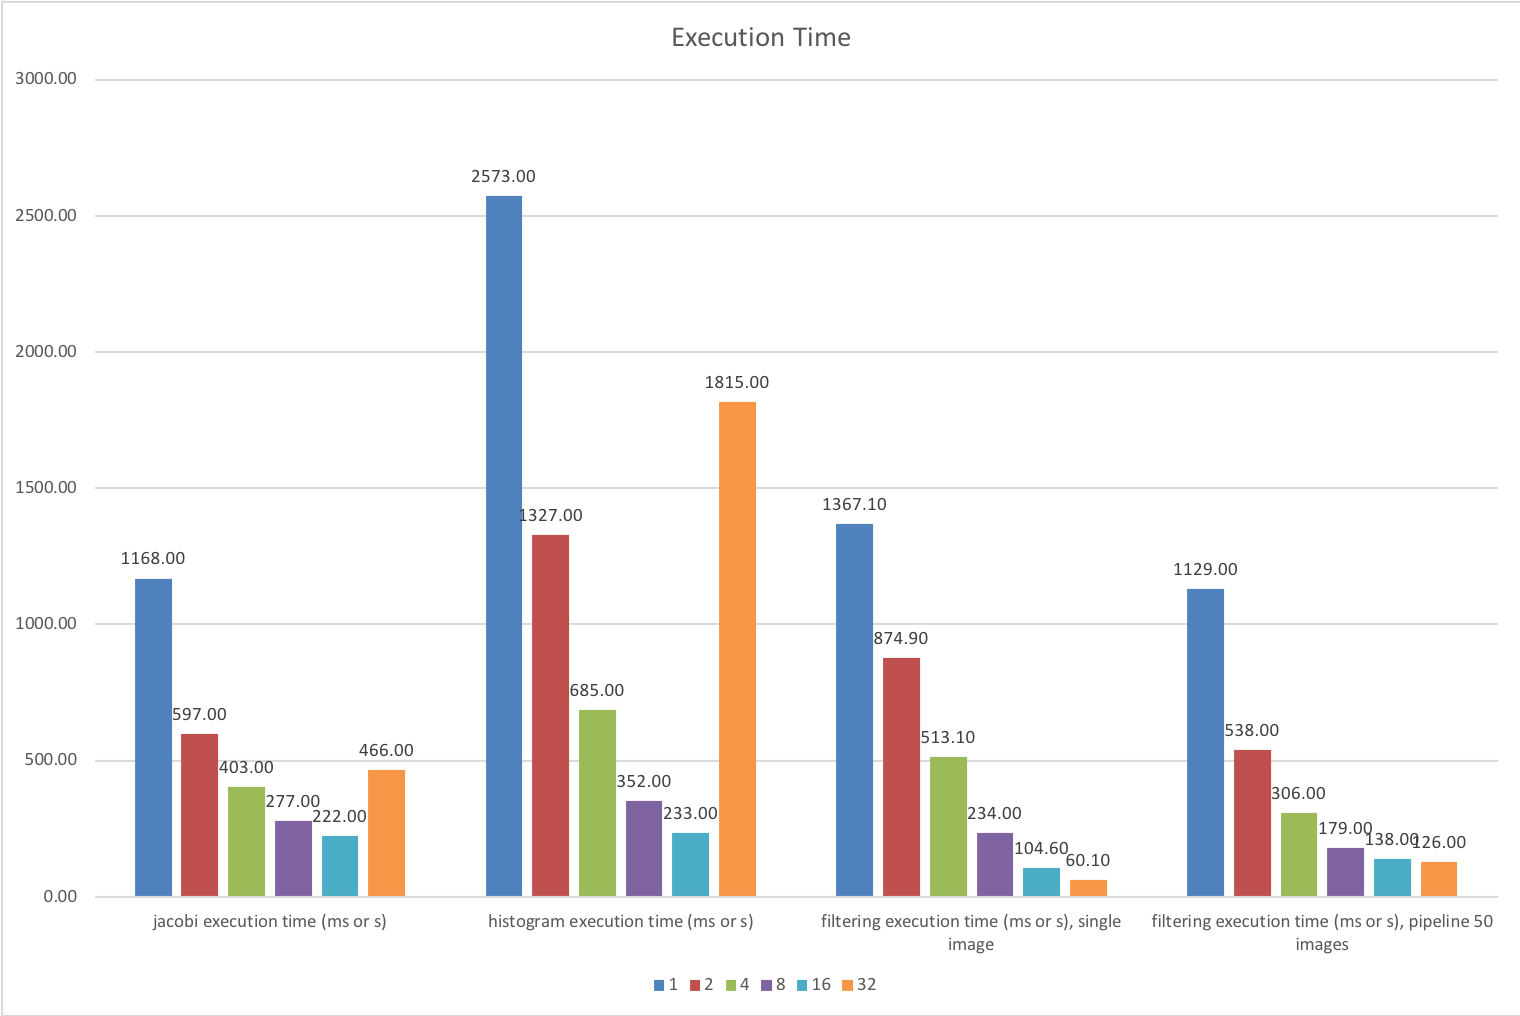
\includegraphics[scale=0.3]{bars.png}}
\vfill
\subfigure[Speedup]{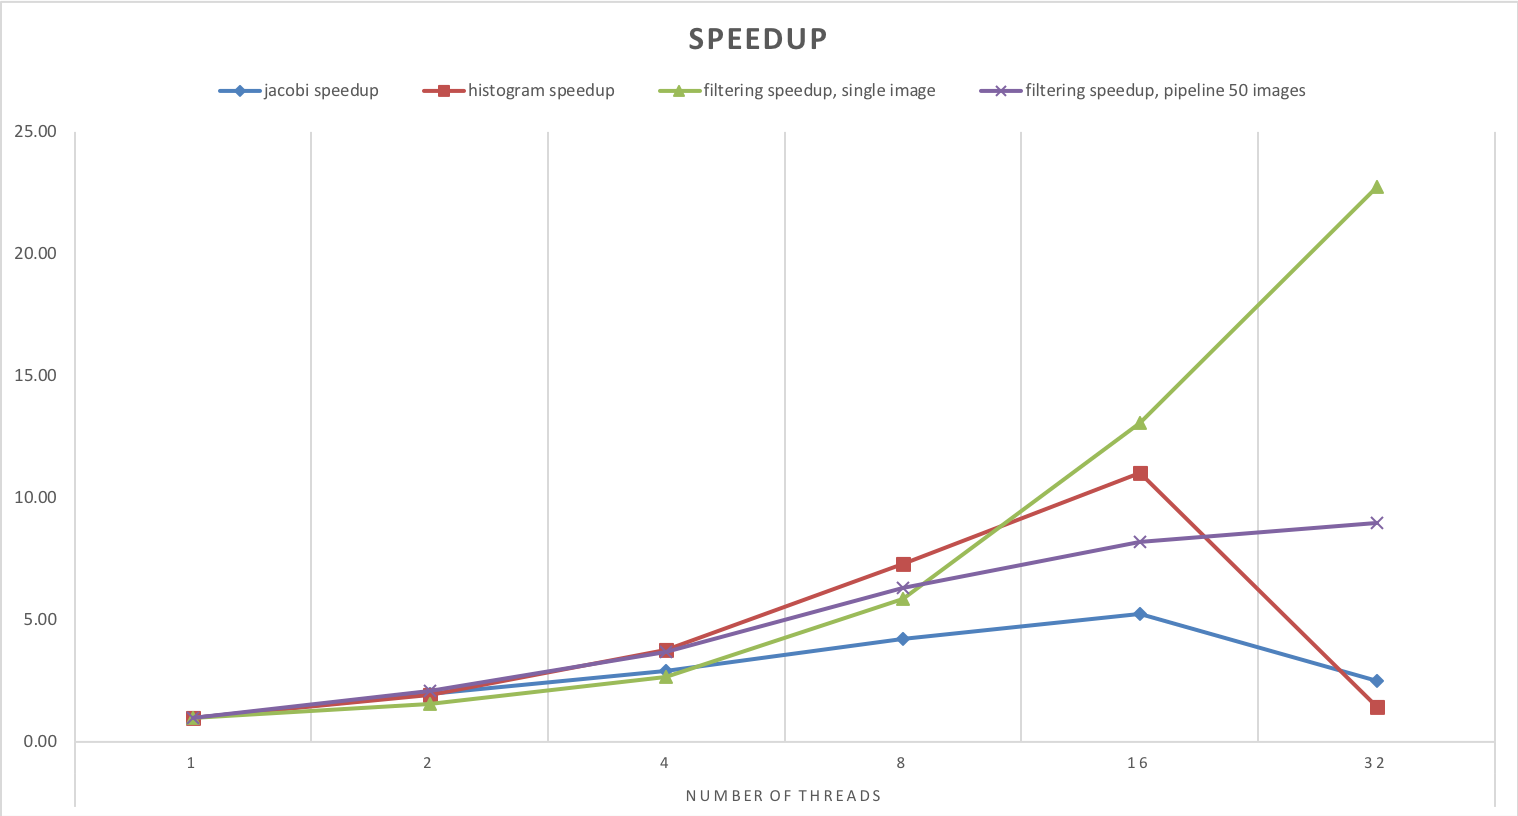
\includegraphics[scale=0.3]{lines.png}}
\caption{Performance Graphs}
\end{figure}


\pagebreak
\begin{verbnobox}[\footnotesize]
Architecture:          x86_64
CPU op-mode(s):        32-bit, 64-bit
Byte Order:            Little Endian
CPU(s):                32
On-line CPU(s) list:   0-31
Thread(s) per core:    1
Core(s) per socket:    16
Socket(s):             2
NUMA node(s):          2
Vendor ID:             GenuineIntel
CPU family:            6
Model:                 79
Model name:            Intel(R) Xeon(R) CPU E5-2683 v4 @ 2.10GHz
Stepping:              1
CPU MHz:               2100.000
BogoMIPS:              4200.29
Virtualization:        VT-x
L1d cache:             32K
L1i cache:             32K
L2 cache:              256K
L3 cache:              40960K
NUMA node0 CPU(s):     0-7,16-23
NUMA node1 CPU(s):     8-15,24-31
\end{verbnobox}



\end{document}
              
            
